



\chapter{Birth death catastrophe -- further results and potential use} 





















\section{Specification of rupture state}
Before we begin, it is important to state a distinction between two varieties of the Birth Death Killing model.
When a rupture event occurrs, the process goes to a state. In the literature, this state is sometimes chosen to be 0, and in other cases there is a seperate rupture state defined, sometimes labeled $R$. The analysis does differ between the two options. And so for clarity, in this document we will refer to the 0 state case as ``killng''; the distinct rupture state as ``catastrophe''.  

\section{Probability Generating Function PDEs}
The probability generating function (PDF),  is defned:
$$G(z,t) = p_0(t) + p_1(t)z + p_2(t)z^2 + p_3(t)z^3 + \dots.$$
The following ODEs can be derivd from the forward Kolmogorov associated with the two processes.

\subsubsection*{Catastrophe}

\begin{equation}
\label{catEq1}
\pdx{G(z,t)}{t} = \big(\beta z^2 - (\beta + \mu + \delta)z + \mu\big)\pdx{G}{z}
\end{equation}

\subsubsection*{Killing}

\begin{equation}
\pdx{G(z,t)}{t} = \delta J(t) +  \big(\beta z^2 - (\beta + \mu + \delta)z + \mu\big)\pdx{G}{z}
\label{killEq1}
\end{equation}

\subsubsection*{Derivation}

It will be sufficient to show a derivation of the ``killing'' equation. The ``catastrophe'' version is similar and simpler. \par

Take the forward Kolmogorov equations: 

$$\begin{cases}
    \ddt{p_i} = \beta (i-1) p_{i-1} + \mu (i+1) p_{i+1} - (\beta + \mu + \delta)ip_i, & i > 0\\
   \\
    \ddt{p_0} = \mu p_1 +  \delta\sum^\infty_{j=1} jp_j.
\end{cases}$$
($p_i = \pr{\xt = i}$, probability the process is in state $i$). In the latter equation with $p_0$, the summation represents all of the possible rupture transitions; from any other state, a collapse to 0 can take place. This summation happens to express the mean; $\mean{\xt}$, which is elsewhere labelled $J(t)$.\par 
In the catastrophe version, since rupture causes transition to a separate state, this summation term is not present, and the first equation will be valid for all $i$.\par
\vspace{10pt}

\noindent
A derivation can be executed by manipulating the equations to fabricate terms containing the PGF, $G(z, t) = \sum^\infty_{i=0}p_i z^i$. It begins by multiplying each side of every $i$th equality by $z^i$. In the case of $i=0$, $z^0 = 1$, so there is no change. 


$$\begin{cases}
    \ddt{p_iz^i} = \beta (i-1) p_{i-1}z^i + \mu (i+1) p_{i+1}z^i - (\beta + \mu + \delta)ip_iz^i, & i > 0\\
   \\
    \ddt{p_0} = \mu p_1 +  \delta J(t).
\end{cases}$$

\noindent
Then, each equation is combined in a sum over all values of $i$ for which there is a positive term.

$$
\sum^\infty_{i=0} \pdx{p_iz^i}{t} = \delta J(t)   + \sum^\infty_{i=0}\lrbs{ \beta (i-1) p_{i-1}z^i + \mu (i+1) p_{i+1}z^i - (\beta + \mu + \delta)ip_iz^i}$$

\noindent
Some rearrangement converts this into 

$$\pdx{}{t}{\sum^\infty_{i=0} p_iz^i } = \delta J(t) + \beta z^2 \sum^\infty_{i=1} ip_iz^{i-1} + \mu\sum^\infty_{i=1}ip_iz^{i-1} - (\beta +\mu+\delta)z\sum^\infty_{i=1}ip_iz^{i-1}$$

\noindent
And since
$$\sum^\infty_{i=1} ip_iz^{i-1}  = \pdx{}{z}\sum^\infty_{i=1} p_iz^{i} = \pdx{G(z,t)}{z},$$
the above, becomes 

$$\pdx{G(z,t)}{t} = \delta J(t) +  \beta z^2\pdx{G}{z}  + \mu\pdx{G}{z} - (\beta + \mu + \delta)z\pdx{G}{z}.$$

\noindent
Equivalent to (\ref{killEq1}).

\section{Identifying the PGFs}

G(z,t), the probability generating function, is a powerful tool for understanding the behaviour of the system and its probable outcomes. Because it can be written as a polynomial sum in which each coefficient is the probability of the process being in a specific state at a given time, valuable information on the process can be extracted. \par
As,
$$G(z,t) = p_0(t) + p_1(t)z + p_2(t)z^2 + p_3(t)z^3 + \dots,$$
The mean, $J(t)$ can be found with $\partial_zG(z,t)|_{z=1}$:
$$\mean{\xt} = p_1(t) + 2p_2(t) + 3p_3(t) + \dots;$$
Individual state-probabilities can be extracted in the following way. Differentiate with respect to $z$, $n$ times,
$$\pdxn{G(z,t)}{z}{n} =  n! \cdot p_n(t) + (n+1)! \cdot p_{n+1}(t) z + \frac{(n+2)!}{2} \cdot p_{n+2}(t) z^2 + \dots,$$
then evaluate at $z=0$ and divide by $n!$:
\begin{equation}
\label{stateFormula}
\frac{1}{n!}\cdot\pdxn{G(z,t)}{z}{n}\bigg|_{z=0} = p_n(t).
\end{equation}
In this way the full dynamic distribution of the system can be elucidated.

Though to do this, we must first obtain the explicit formula $G(z,t)$. There will be some difference between the two cases, but the process is similar --- both (\ref{catEq1}) and (\ref{killEq1}) can be solved with the method of characteristics. 


\subsection{Method of characteristics}

Generally, first order, linear PDEs of the type we are dealing can be solved as a family of ODEs. The method begins by introducing a change of variables $(z,t)\to(s,\tau)$;
$$G(z,t)\equiv G\lrb{z(s, \tau),t(s,\tau)} = G(s, \tau).$$
It proceeds by seeking solutions on characteristic lines of constant $s$: $G(\tau)$. An initial curve must be fixed, from which these solutions will progress. The selection is somewhat arbitrary; many options will work, though a good choice can keep the analysis more simple. There are some hard conditions. For example, the initial line must not be parallel in the $s,$ $\tau$ space to the progressing solutions. In cases such as ours, it is often appropriate to use
\begin{align}
\label{ICs}
z(s,0) = s&& t(s,0) = 0
\end{align}
\subsubsection*{Catastrophe}
Assuming the probability generating function changes with only  one variable --- $G(\tau(z, t))$ --- we can write down the characteristic equations as ODEs. First, consider
\begin{equation*}
\dda{G}{\tau} =  \lrbc{\dda{t}{\tau}}  \pdx{G}{t}+ \lrbc{\dda{z}{\tau} }\pdx{G}{z}.
\end{equation*}
Comparing with the catastrophe equation, (\ref{catEq1}), there is a similarity,
$$0=  \lrbc{- 1}\pdx{G}{t} + \lrbc{\beta z^2 -( \beta + \mu + \delta)z + \mu} \pdx{G}{z},$$
and we can extract the three characteristic ODEs:
\begin{align*}
\label{Char1}
\dda{G}{\tau} = 0,&& \dda{t}{\tau} = -1, && \dda{z}{\tau} = \beta z^2 - (\beta + \mu + \delta)z + \mu.
\end{align*}
The first of these, which will differ in the killing case, tells us that  
$$G = \phi{(s)},$$
$\phi$ constant on curves of unchanging $s$.\par
In both cases, the initial condition on $G$ will be $$G(z, 0) = z$$ because starting with a single individual means $p_1(0) =1$ and $p_{i\neq1}(0) = 0$. Therefore, $G = \phi{(s)}$ in conjunction with our choice of initial curve, $z(s, 0) = s$, allows $\phi(s)$ to be fixed as $s$;
$$G(s,\tau) = s.$$\par

\noindent
Moving to the second characteristic ODE:
$$\dda{t}{\tau} = -1 \hspace{5pt} \implies \hspace{5pt} t = -\tau +  C_1(s) \text{  (constant for unchanging }s ).$$
Our initial condition, $t(s,0) = 0$ fixes $C_1(s) = 0$, so $t = -\tau$.\par
The remaining characteristic equation with $z$ happens to be the same form as an ODE describing the no-rupture probability, $I(t)$. 
\begin{equation}
\label{char3cat}
\dda{z}{\tau} = \beta z^2 - (\beta + \mu + \delta)z + \mu
\end{equation}
What differs is the initial condition. In the case of, $I(t)$, at time 0 it is 1 --- rupture having definitely not occurred; with $z(s,t)$, our chosen initial condition is $z(s, 0) = s$. Hence, the solution to (\ref{char3cat}) is very similar to the formula for $I(t)$, though in places where there is seen a one, here an $s$ is found:
\begin{equation*}
z = \frac{a(s-b) - b(s-a)\ee^{\beta(a-b) \tau} } {(s-b) - (s-a)\ee^{\beta(a-b) \tau}}
\end{equation*}
also, In this it is $\tau$ rather than $t$.\par
Since $G(z, t) = s(z, t)$, we can obtain the final solution in one step: Rearrange the above for $s$, and place $-t$ at each $\tau$. By a happenstance of symmetry, this turns out looking quite the same:
\begin{equation}
\label{s2343}
s = \frac{a(z-b) - b(z-a)\ee^{\beta(a-b) t} } {(z-b) - (z-a)\ee^{\beta(a-b) t}}.
\end{equation}
And so we have it, by the somewhat dark art of characteristics, the probability generating function emerges as
\begin{equation*}
G(z,t) = \frac{a(z-b) - b(z-a)\ee^{\beta(a-b) t} } {(z-b) - (z-a)\ee^{\beta(a-b) t}}.
\end{equation*}
As will be seen, in obtaining the state probabilities via repeated partial differentiation in $z$, it is advantageous to write the formula as
\begin{equation*}
G(z,t) = \frac{ab(1-\ee^{\beta(a-b) t}) - z(a-b\ee^{\beta(a-b) t}) } {  (b-a\ee^{\beta(a-b) t}) -z(1-\ee^{\beta(a-b) t})  }
\end{equation*}
For now, let us move on to the modification that is introduced in the killing case. 


\subsubsection*{Killing}

When rupture collapses the process to 0, it may have happened at any positive state.  As we've seen, because of this, the forward Kolmogorov equation describing $p_0(t)$ includes a separate term related to every natural number. Thankfully, these do compress neatly into an expression of the mean, $\mean{\xt} = J(t)$. Hence, in the PDE, (\ref{killEq1}), there is an inhomogeneous term: $\delta J(t)$.\par
Making the same comparison as in the catastrophe case, 

\begin{align*}
\dda{G}{\tau} &=  \lrbc{\dda{t}{\tau}}  \pdx{G}{t}+ \lrbc{\dda{z}{\tau} }\pdx{G}{z}\\
-\delta J(t)&=  \lrbc{- 1}\pdx{G}{t} + \lrbc{\beta z^2 -( \beta + \mu + \delta)z + \mu} \pdx{G}{z}
\end{align*}
we see the characteristic equations are largely the same, just that the first picks up this extra component: 
\begin{align*}
\label{Char2}
\dda{G}{\tau} = -\delta J(-\tau),&& \dda{t}{\tau} = -1, && \dda{z}{\tau} = \beta z^2 - (\beta + \mu + \delta)z + \mu.
\end{align*}

%last 2 the same

%first:

\noindent
From previous work, we know 
$$-\delta J(t) = \ddt{I(t)}.$$
Simply because $\dd t = -\dd \tau$, it follows that 
$$\delta J(-\tau) = \dda{I(-\tau)}{\tau}.$$
And so, looking to the first characteristic equation, 
$$\dda{G}{\tau} = \dda{I(-\tau)}{\tau},$$
hence,
$$G(s,\tau) = -I(-\tau) + \phi(s).$$
Again, with some $\phi$ stationary for over constant $s$. \par
With the initial condition, $G(z, t=0) = z(s, \tau = 0) = s$,
$$G(s,0) =s= -I(0) + \phi(s),$$
$\phi$ can be fixed: $\phi(s) = 1 + s;$
$$G(s,\tau) = 1 - I(-\tau) + s.$$\par
Identical to the catastrophe case, the final characteristic equation is solved in the same way for the same result, (\ref{s2343}). So finally, 
$$G(z,t) = 1 - I(t)  + \frac{ab(1-\ee^{\beta(a-b) t}) - z(a-b\ee^{\beta(a-b) t}) } {  (b-a\ee^{\beta(a-b) t}) -z(1-\ee^{\beta(a-b) t})  }.$$
And this result makes good sense. With $1 - I(t)$ being the likelihood that the process has made the ``killing'' transition to 0, these two terms stand to complement the probability that state $0$ is reached from individual death (this component arises from the final term). 


\section{State probabilities}

Using formula (\ref{stateFormula}), we can obtain the individual state probabilities. The first, $p_0(t)$ will differ between the catastrophe and killing cases: 
$$G(0 , t) = \begin{cases}
\frac{ab(1-\ee^{\beta(a-b) t})  } {  (b-a\ee^{\beta(a-b) t})   }, & \text{(catastrophe)}\\
1 - I(t) + \frac{ab(1-\ee^{\beta(a-b) t})  } {  (b-a\ee^{\beta(a-b) t})   }, & \text{(killing).}
\end{cases}$$
As stated above, the fraction term in each case represents the probability of reaching 0 by death, and the $1-I(t)$ pertains to reaching 0 by collapse in ``killing''.\par 
From here, the state probabilities, $p_1(t)$, $p_2(t)$, $p_3(t)\dots$, do not differ between the cases. Repeated differentiation of $G(z,t)$ with respect to $z$ reveals the formula,
$$\frac{\partial^n G}{\partial z^n} =n! \ee^{\beta(a-b)t}(a-b)^2  \frac{\lrb{1-\ee^{\beta(a-b)t}}^ {n-1} }{\lrb{b - a\ee^{\beta(a-b)t} - \lrb{1-\ee^{\beta(a-b)t}}z} ^ {n+1}} $$
Hence, setting $z=0$, and dividing by $n!$, the state probabilities for $n\geq1$ are described by,
\begin{equation}
\label{stateprob}
p_n(t) =\lrb{ \frac{ a-b }{{b - a\ee^{\beta(a-b)t}}}}^2 \ee^{\beta(a-b)t} \lrb{\frac{{1-\ee^{\beta(a-b)t}}}{{b - a\ee^{\beta(a-b)t}} } }^{n-1}.
\end{equation} 

\section{Quasi-stationary distribution }

\cite{van2011quasi}.  Both the BDC and BDK processes are subject to eventual absorption --- either at the designated rupture state, or by death, at 0. But suppose there is an example of a particular realisation which has, by chance, not yet reached fixation. It continues, increasingly against the odds as time marches on... How has it managed this? If it flies too low, depletion to zero becomes more and more probable; but, almost as bad, if it flies high, a population booming in number, there are all the more opportunities for its downfall, a crashing and ceasing to be.
Like Icarus, the process which does not fall into the sea does so by hovering at some appropriate height; 

its wings neither undermined by the spray of a hungry ocean, nor by the beating rays of the sun at a rarified altitude. \par
In such terms, we can examine this rogue process as it goes on to defy all odds. Its fate will tend to be predicted by the quasi-stationary distribution. This, a set of limiting conditional probabilities, each qualified by non-fixation.\par
Define the probability of fixation: $F(t)$. That is, either by death or collapse. The conditional state probabilities can be computed by,
$$\pr{\xt = i} = \pr{\xt=i| \text{ at fixation}}F(t) + \pr{\xt=i| \text{ non-fixation}} \lrb{1-F(t)}.$$
Ignoring, for now, the case of $i = 0$ \& $i = R$, $\xt$ has reached absorption, $\pr{\xt = i} = 0$. Hence,
 $$\pr{\xt = i} =  \pr{\xt=i| \text{ non-fixation}} \lrb{1-F(t)},$$
and it follows that,
$$\pr{\xt=i| \text{ non-fixation}} = \frac{\pr{\xt = i} }{1-F(t)}.$$
With the state probabilities known (\ref{stateprob}), 
There is a question of what form $F(t)$ takes, and how it differs between the two BDK and BDC. When $\mu=0$, the non-fixation probability of both cases is defined by $I(t)$, i.e. $F(t) = 1-I(t)$.





\begin{figure}[H]
    \centering
    % First figure
    \begin{subfigure}{0.47\textwidth}
        \centering
        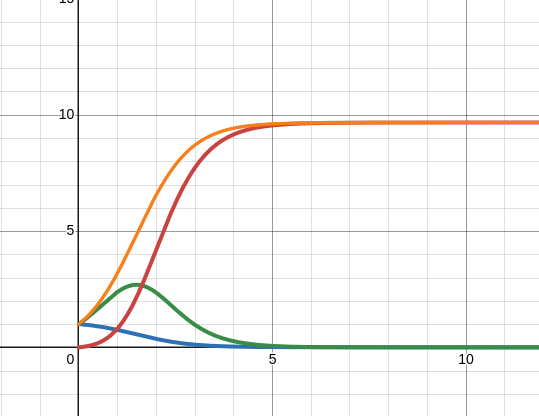
\includegraphics[width=\textwidth]{chapter5/IMG_ch5/QSmean/QS1} % Adjust the image path as necessary
        \caption{When $\mu = 0$.}
        \label{fig:figure1}
    \end{subfigure}
    \hspace{\fill} % Optional: adds space between figures
    % Second figure
    \begin{subfigure}{0.47\textwidth}
        \centering
        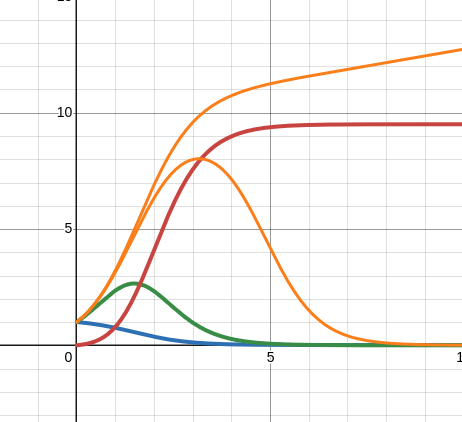
\includegraphics[width=\textwidth]{chapter5/IMG_ch5/QSmean/QS2} % Adjust the image path as necessary
        \caption{When $\mu > 0$.}
        \label{fig:figure2}
    \end{subfigure}
    
    \caption{In the image on the right, the conditional mean (yellow) going up at late time is the mean conditioned on $\xt \neq0$: $J(t)/\hat I(t)$. The yellow line tending to 0 is for the mean conditioned on non-catastrophe $\mean{\xt|\xt \neq R}$}
    \label{fig:two_figures}
\end{figure}



Considering the no-death $\mu = 0$ case on the left above,  it can be easily seen that the conditional mean (yellow) tends to the same limit as $V(t)$, which is shown in red.  That is 

$$\lim_{t\to\infty}     \frac{J(t)}{I(t)}     =    \lim_{t\to\infty} V(t)  = 1 + \frac{\lambda}{\delta}.$$

Here,  when $\delta$ shrinks to 0, the QS mean and expected release count tend to infinity.  








\section{Burst size distribution}

Using 

$$ \int p_k(t)\dd t  = (n\beta)^{-1} \lrb{\frac{{1-\ee^{\beta(a-b)t}}}{{b - a\ee^{\beta(a-b)t}} } }^{n},$$

the following equation can be approached. 


$$\pr{K = k} = \delta k \int_0^\infty p_k(t)\dd t$$
Where $p_k(t) = \pr{\xt = k}$. We have above determined that 

$$p_k(t) =\lrb{ \frac{ a-b }{{b - a\ee^{\beta(a-b)t}}}}^2 \ee^{\beta(a-b)t} \lrb{\frac{{1-\ee^{\beta(a-b)t}}}{{b - a\ee^{\beta(a-b)t}} } }^{k-1}.$$
Then, we have the formula

$$\pr{K = k} = \delta k \int_0^\infty p_k(t)\dd t$$
The current goal is to verify this using Gillespie algorithm simulations. First, we have the integration,

$$\int p_k(t)\dd t  = (k\beta)^{-1} \lrb{\frac{1 - \ee^{\beta(a-b)t}}{b - a\ee^{\beta(a-b)t}}}^k $$
Which can be verified with reverse differentiation (found with Wolfram Alpha). With this,

$$\pr{K=k} = \frac{\delta}{\beta}\lrbs{ \lrb{\frac{1 - \ee^{\beta(a-b)t}}{b - a\ee^{\beta(a-b)t}}}^k}^\infty_0 = \frac{\delta}{\beta}\lrb{\frac{1}{a}}^k$$

$$\pr{K=k} = \frac{\delta}{\beta}\lrb{\frac{1}{\frac{\beta+\mu+\delta}{2\beta} + \sqrt{\lrb{\frac{\beta+\mu+\delta}{2\beta}}^2 - \frac{\mu}{\beta}}}}^k$$






\section{Further considerations}

From 
\begin{align}
\mean{K} &= \mean{K| \tau > t} \pr{\tau > t} + \mean{K| \tau < t}\pr{\tau<t},\\
&= \mean{K|\tau > t} I(t) + \frac{V(t)}{1 - I(t)} \lrb{1 - I(t)},
\end{align}
We find,
$$\mean{K| \tau > t}  = \frac{\mean{K} - V(t)}{I(t)}   =   \frac{  \sum^{\infty}_{k} k \pr{K = k}  - V(t)}{I(t)}$$

Note: $\mean{K} = V_{\text{inf}} = \frac{\lambda - \mu}{\delta} \lrb{1 - I_-} + 1$ (check). Actually, there is some complication. $V(t) = \mean{\yt}$ where $\yt$ is the number of agents ``released''. Basically, at the rupture event, the value of $\xt$ immediately before catastrophe becomes the value of $\yt$. $\yt$ is otherwise 0. What I'm getting at is that $V(t\to \infty)$ does not only represent the average burst size. When $\mu > 0$, some processes will go extinct without catastrophe. In these cases, $\yt$ will remain 0. $V(t) = \mean{\yt}$ captures these processes in its quantity. So if we want to extract the true burst size mean from $V(t)$, we must somehow condition on the processes that did reach rupture. 

$$V(t) = \mean{\yt}$$ 
Whether the catastrophe event has taken place or not can be represented by the truth of $\yt>0$, as the minimum burst size is 1. Rupture has occurred with probability $1 - I(t)$.
$$\mean{\yt} = \mean{\yt|\yt > 0}(1-I(t)) + {\mean{\yt | \yt = 0}}I(t)$$
Since $ {\mean{\yt | \yt = 0}} = 0,$
$$\mean{\yt} = \mean{\yt|\yt > 0}(1-I(t))$$
$$ \mean{\yt|\yt > 0} = \frac{\mean{\yt}}{1-I(t)}.$$
This can be thought of as $\mean{\text{Burst size } | \text{ burst has happened}}$. Note equivalence to a term written above:
$$\mean{K | \tau < t} =\frac{V(t)}{1-I(t)}. $$
So, the overall expected burst size --- the expected size of an arbitrarily generated burst --- is the late time value of this expression: 
$$\mean{K} = \lim_{t\to \infty} \lrb{\mean{K| \tau < t}} = \frac{V_{\text{inf}}}{1 - I_-}.$$
$$\mean{K} = \frac{\frac{\lambda - \mu}{\delta}(1-I_-) + 1}{1-I_-} = \frac{\lambda - \mu}{\delta} + \frac{1}{1-I_-}.$$

Hence, 
$$\mean{K|\tau > t} = \frac{\frac{V_{\text{inf}}}{1 - I_-} - V(t)}{I(t)} =  \frac{\frac{\lambda - \mu}{\delta} + \frac{1}{1-I_-} - V(t)}{I(t)}.$$

Though, there is a curious circularity to this which I'm yet to fully understand. Look what happens when we take $\mean{K|\tau> t}$ at its late time value. 

$$\lim_{t\to\infty}\mean{K|\tau > t} = \frac{\frac{V_{\text{inf}}}{1 - I_-} - V_{\text{inf}}}{I_-}  = \frac{V_{\text{inf}}}{1 - I_-} = \mean{K}$$
Maybe this is an obvious result, but I am yet to fully grasp why.













\section{Potential application in BMVR}




\noindent
Consider a reasonably large population of cells initially infected all by a single \ft $\; $bacteria. Over time, each cell acts independently as a birth death catastrophe process described by the usual quantities, $J$ and $I$. Say there were $N_0$ of such cells at the beginning; as the model progresses there will be approximately $N_0 I(t)$ cells which are yet to rupture. This estimate becoming increasingly accurate with progressively larger $N_0$.\par
In previous work, the quantity, $V(t)$, has been used to describe the count of bacteria released from a single cell. In that application, it has been found to increase at a rate proportional to the second moment of intracellular count, $\delta \mean{\xt^2}$. In this case of $N_0$ initially infected cells, there doesn't seem to be an issue with the same quantification being used --- there being $\Vt(t) = N_0 V(t)$ extracellular bacteria through time (assuming no reabsorption or replication in the extracellular population).\par 

\subsubsection*{Proportional release formula}

But I'm curious about another way $\Vt$ might be quantified. As a starting point, suppose $N_0$ is very large, and that we begin observing the model at a reasonably late start-time, $t_s$. Late enough for convergence to the quasi-stationary distribution in $\xt$. We have previously computed this limiting conditional distribution and its mean: $\mean{\xt | \xt\notin\{R, 0\}}_{t\to\infty}$ and $\pr{\xt = k | \xt\notin\{R, 0\}}_{t\to\infty}$. \par
Through this period of time, it seems the rate of extracellular release, $\dd \Vt/ \dd t$, should be made up of the number of infected cells remaining, $N_0 \hat I(t_s + t)$, ($\hat I $ being the non-fixation probability), multiplied by the expected number in each cell, $\mean{\xx_{t_s + t} | \xx_{t_s + t}\notin\{R, 0\}}_{t\to\infty}$.

$$\ddt{\Vt} = N_0 \hat I(t_s + t) \cdot \mean{\xx_{t_s + t} | \xx_{t_s + t}\notin\{R, 0\}}_{t\to\infty}$$


\noindent
(for $t> t_s$, the stationarity time). In principle, we might be able to compute $\Vt$ in this way.\par
There is an apparent issue with this arrangement, which is: at late time, as the mean bacterial count becomes stationary, it is also true that the non-fixation probability tends towards 0. This could be mitigated by assuming $N_0$ is sufficiently large. Or, say for example we don't know when the infection began, or how many bacteria it started with. But suppose we do know the current concentration of infected cells in the blood, and, we know the infection has been going on long enough for contents of remaining infected cells to be near the stationary distribution. (Of course, this now assumes reabsorption). In this case, the infected cell count, $N_0 \hat I(t_s + t)$, would be taken as a constant --- call it $\Ic$. And, the factor multiplying it in the release rate would merely be the QS mean (which we have a formula for):

$$\ddt{\Vt} = \Ic\cdot \mean{\xx_{t} | \xx_{t}\notin\{R, 0\}}_{t\to\infty}$$

Important to recognise this now assumes reabsorption, but say we roll with the idea.


\subsubsection*{Intuitive argument}

By some intuitive logic of this kind,  it may be feasible to propose a small update to the ``basic model of viral replication'':\par
From this,

\begin{align*}
\ddt{I} &= \beta T V - \delta I\\
\ddt{V} &= p I - c V
\end{align*}


\noindent
to this,

\begin{align*}
\ddt{I} &= \beta T V - \delta I\\
\ddt{V} &= \lrbs{\mean{\xx_{t} | \xx_{t}\notin\{R, 0\}}_{t\to\infty}} I - c V
\end{align*}


\noindent
Where the only difference is that the constant viral release rate, $p$, has been replaced by a slightly more complicated constant value which is a combination of intra-cellular rates.

$$p = \mean{\xx_{t} | \xx_{t}\notin\{R, 0\}}_{t\to\infty} =\quad ?$$ 


\noindent
The purpose of this is that, given someone is in a situation where they have a good estimate for $p$, the viral release rate, by our logic, they may then be able to access an approximation for the rates constituting the QS mean. \par

\vspace{15pt}


\noindent
(need to look up the formula for QS mean, but its something like $\lim_{t\to\infty}{J(t) / (1-\hat I(t))}$. I think there is an important point around whether $\mu = 0$ or not.)


\subsubsection*{Towards a correction}

The above formula is incorrect, but there might be a way to fix it. The problem is that the burst rate depends on intracellular load.


We can use the approximation which assumes that the distribution of cell infection sizes is at its late-time stationary value. Or maybe this isn't the best option. Because at any time, there will be infected cells that begin their infection dynamics at a number of different start times. The distribution of release times is given by a known formula. So Perhaps there is some way of combining this time pdf and the second-moment formula conditional on time in a normalization. 

Is it an integral:

$$p =  \delta \int \phi(t) \mean{\xt^2 | \xt \notin \{R, 0 \} }(t)  \dd t$$

(The second moment conditional on non-rupture, normalized over the probability density of burst times ) Where $\phi(t)$ is the known pdf of rupture times. \par
Or is it this:


$$p = \int \phi(t) \mean{R | \tau = t} \dd t$$

(The rupture size probability given burst time, normalized over the probability density of burst times)


\subsubsection*{Iterating cycles --- overall expected release rate?}
The quantity this is trying to represent can be thought of simply as follows. Consider a model where at first there is a single infected macrophage. When it ruptures, each of the output bacteria go on to found a new BDC process in a new infected cell. Until, at different times, each of these ends in turn and cycles continue with new intracellular infectious processes beginning and ending, beginning and ending.\par

Over a sufficient period of time following the initial cell, there will emerge a sort of stationarity whereby any given release event will exhibit a burst time and burst size according to the known distributions. Short-duration processes will by nature occur more frequently than longer-duration ones. 


{ What we desire is an overall rate of release events and their sizes to make up an approximation to replace the} $p I $ {term in the Basic Model of Viral Replication above.}


{For any given cell, the probability that it will burst soon will be higher if it has a high internal census. But large bursts, in this population cyclic dynamic will be less frequent because short release times with smaller bursts happen with a greater frequency. }








































